\chapter{Navigation and Guidance Domain Chapter}
\label{ch:domain-navigation}

Navigation remains shadow-synthetic: the adapter and replay harness show architectural portability, but the evidence is not yet strong enough for promotion because the row still depends on bounded synthetic traces.

\section{{Domain problem}}
Navigation systems must preserve corridor, obstacle, or path-feasibility constraints even when localization and guidance telemetry degrade under dropout or stale updates.

\section{{Degraded-observation hazard}}
The ORIUS book forces every domain through the same hazard lens: the runtime does not act
on the true state directly; it acts on a degraded, delayed, or otherwise imperfect
observation surface.  The row is only credible if the gap between those two surfaces can
be expressed, replayed, repaired, and audited explicitly.
The current row includes synthetic dropout, stale localization, corrupted headings, and delayed guidance packets.

\section{{ORIUS instantiation}}
The navigation adapter maps localization and path telemetry to the universal kernel, but the current row remains a portability and closure surface rather than a real-data proof surface.

\section{{Safety object}}
The defended predicate is bounded true-state path violation under degraded observation, expressed as corridor or guidance-envelope violation rather than battery-style state-of-charge semantics.

\section{{Dataset and training surface}}
The row is intentionally flagged as synthetic in the closure matrix and is treated as portability evidence rather than parity evidence.
The chapter-local evidence packet is intentionally tied to locked artifacts rather than to
narrative memory.  Table~\ref{tab:ch40-44-cross-domain-support} gives the shared cross-domain
support layer for compiled Chapters~40--44, while the table below isolates the current row.

\section{{Feature, split, and training protocol}}
Navigation is shown here as a portability row, not as a defended forecasting row. The chapter still exposes the expected feature/split/training interface so the real-data closure work has an exact manuscript target once the KITTI-backed row is complete.

\IfFileExists{paper/assets/tables/generated/tbl_navigation_training_surface.tex}{%
\begin{table}[htbp]
\centering
\small
\caption{Navigation and Guidance training and data surface for the compiled chapter evidence block.}
\label{tab:navigation-training-surface}
\begin{tabular}{p{0.31\linewidth}p{0.61\linewidth}}
\toprule
\textbf{Field} & \textbf{Value}\\
\midrule
Raw/data gate & blocked\\
Feature surface & synthetic portability harness only\\
Split counts & train n/a / calibration n/a / validation n/a / test n/a\\
Primary target & corridor or guidance-envelope violation\\
Forecast metrics & n/a until the real-data navigation row is locked\\
Verification state & adapter portability passes, but the defended train/validate chain is blocked\\
Artifact lineage & reports/publication/orius\_equal\_domain\_parity\_matrix.csv; reports/universal\_orius\_validation/domain\_closure\_matrix.csv\\
\bottomrule
\end{tabular}
\end{table}
%
}{%
\begin{table}[htbp]
\centering
\small
\caption{Navigation and Guidance training and data surface for the compiled chapter evidence block.}
\label{tab:navigation-training-surface}
\begin{tabular}{p{0.31\linewidth}p{0.61\linewidth}}
\toprule
\textbf{Field} & \textbf{Value}\\
\midrule
Raw/data gate & blocked\\
Feature surface & synthetic portability harness only\\
Split counts & train n/a / calibration n/a / validation n/a / test n/a\\
Primary target & corridor or guidance-envelope violation\\
Forecast metrics & n/a until the real-data navigation row is locked\\
Verification state & adapter portability passes, but the defended train/validate chain is blocked\\
Artifact lineage & reports/publication/orius\_equal\_domain\_parity\_matrix.csv; reports/universal\_orius\_validation/domain\_closure\_matrix.csv\\
\bottomrule
\end{tabular}
\end{table}
%
}

\section{{Replay and evidence surface}}
ORIUS reduces the synthetic-row TSVR materially, but not to zero, which is why the book treats navigation as an architecture-validating row rather than a defended empirical peer.

\IfFileExists{paper/assets/tables/generated/tbl_navigation_replay_surface.tex}{%
\begin{table}[htbp]
\centering
\small
\caption{Navigation and Guidance replay, runtime, and promotion surface for the compiled chapter evidence block.}
\label{tab:navigation-replay-surface}
\begin{tabular}{p{0.31\linewidth}p{0.61\linewidth}}
\toprule
\textbf{Field} & \textbf{Value}\\
\midrule
Governing replay metric & baseline TSVR 0.6667 -> ORIUS TSVR 0.2500\\
Replay status & pass\\
Safe-action soundness & blocked\_real\_data\_gap\\
Fallback semantics & hold\_position / bounded\_runtime\_pass\\
CertOS lifecycle & gated / gated\\
Multi-agent portability & gated / gated\\
Evidence tier & shadow\_synthetic\\
Exact blocker & navigation\_real\_data\_gap\\
Artifact lineage & reports/publication/orius\_domain\_closure\_matrix.csv; reports/universal\_orius\_validation/domain\_closure\_matrix.csv; reports/publication/orius\_equal\_domain\_parity\_matrix.csv\\
\bottomrule
\end{tabular}
\end{table}
%
}{%
\begin{table}[htbp]
\centering
\small
\caption{Navigation and Guidance replay, runtime, and promotion surface for the compiled chapter evidence block.}
\label{tab:navigation-replay-surface}
\begin{tabular}{p{0.31\linewidth}p{0.61\linewidth}}
\toprule
\textbf{Field} & \textbf{Value}\\
\midrule
Governing replay metric & baseline TSVR 0.6667 -> ORIUS TSVR 0.2500\\
Replay status & pass\\
Safe-action soundness & blocked\_real\_data\_gap\\
Fallback semantics & hold\_position / bounded\_runtime\_pass\\
CertOS lifecycle & gated / gated\\
Multi-agent portability & gated / gated\\
Evidence tier & shadow\_synthetic\\
Exact blocker & navigation\_real\_data\_gap\\
Artifact lineage & reports/publication/orius\_domain\_closure\_matrix.csv; reports/universal\_orius\_validation/domain\_closure\_matrix.csv; reports/publication/orius\_equal\_domain\_parity\_matrix.csv\\
\bottomrule
\end{tabular}
\end{table}
%
}

\begin{figure}[htbp]
\centering
\IfFileExists{reports/publication/fig_navigation_chapter_snapshot.png}{%
\includegraphics[width=0.90\textwidth]{reports/publication/fig_navigation_chapter_snapshot.png}%
}{%
\includegraphics[width=0.90\textwidth]{../reports/publication/fig_navigation_chapter_snapshot.png}%
}
\caption{Navigation and Guidance replay snapshot derived from the governed domain-closure artifact. Baseline and repaired TSVR are taken from the locked closure matrix; tier and blocker language remain governed by the parity gate.}
\label{fig:navigation-chapter-snapshot}
\end{figure}

\section{{Fallback and runtime behavior}}
Navigation currently falls back to hold-position or bounded low-aggression guidance, but that behavior remains portability-level until the real-data row is complete.

\section{{Evidence tier and promotion blocker}}
The chapter is intentionally explicit about its weaker status. The navigation adapter travels through the shared ORIUS runtime, the replay harness runs, and the runtime fallback semantics are legible, but the defended train/validate/replay chain is still blocked by the missing real-data row recorded in the parity matrix.


\IfFileExists{paper/assets/tables/generated/tbl_navigation_promotion_obligations.tex}{%
\begin{table}[htbp]
\centering
\small
\caption{Promotion obligations that remain open for navigation and guidance before the parity gate can be widened.}
\label{tab:navigation-promotion-obligations}
\begin{tabular}{p{0.24\linewidth}p{0.20\linewidth}p{0.44\linewidth}}
\toprule
\textbf{Obligation} & \textbf{Current state} & \textbf{What must happen next}\\
\midrule
Real raw-source contract & blocked\_real\_data\_gap & Install the canonical KITTI-backed real-data row under data/navigation/raw/kitti\_odometry/ or the optional ORIUS\_EXTERNAL\_DATA\_ROOT fallback and retire synthetic fallback from the defended path.\\
Deterministic processed/train chain & blocked\_real\_data\_gap & Produce a locked navigation\_orius.csv, verified splits, model bundle, uncertainty outputs, and backtests from the real-data row.\\
Replay and safe-action soundness & blocked\_real\_data\_gap & Re-run universal replay and soundness checks on the real row so promotion is governed by the same closure matrix as the defended domains.\\
Parity promotion artifact & shadow\_synthetic & Update the parity and closure artifacts only after the real-data train/validate/replay chain passes end to end.\\
\bottomrule
\end{tabular}
\end{table}
%
}{%
\begin{table}[htbp]
\centering
\small
\caption{Promotion obligations that remain open for navigation and guidance before the parity gate can be widened.}
\label{tab:navigation-promotion-obligations}
\begin{tabular}{p{0.24\linewidth}p{0.20\linewidth}p{0.44\linewidth}}
\toprule
\textbf{Obligation} & \textbf{Current state} & \textbf{What must happen next}\\
\midrule
Real raw-source contract & blocked\_real\_data\_gap & Install the canonical KITTI-backed real-data row under data/navigation/raw/kitti\_odometry/ or the optional ORIUS\_EXTERNAL\_DATA\_ROOT fallback and retire synthetic fallback from the defended path.\\
Deterministic processed/train chain & blocked\_real\_data\_gap & Produce a locked navigation\_orius.csv, verified splits, model bundle, uncertainty outputs, and backtests from the real-data row.\\
Replay and safe-action soundness & blocked\_real\_data\_gap & Re-run universal replay and soundness checks on the real row so promotion is governed by the same closure matrix as the defended domains.\\
Parity promotion artifact & shadow\_synthetic & Update the parity and closure artifacts only after the real-data train/validate/replay chain passes end to end.\\
\bottomrule
\end{tabular}
\end{table}
%
}

\section{{Limitations and exact non-claims}}
No claim of field-grade navigation validation should be made from the current row. This row does not claim field-validated navigation safety; it remains an architectural portability and protocol-design surface until real telemetry closes the gap.

The current promotion obligation for this row remains explicit: Promotion requires locked real-data navigation telemetry, verified replay surfaces, and the same certificate semantics enforced elsewhere in the book.
